% generated by doc/figures.py -- edit the script, not this file
\begin{tikzpicture}[thick, every node/.style={font=\small}]
  % ((a b) c) -> d, coupled through e
  \node (a) at (0,0) {$a$};
  \node (b) at (0.9,0) {$b$};
  \node[circle, fill, inner sep=1.6pt] (v1) at (0.45,0.75) {};
  \node (c) at (1.8,0) {$c$};
  \node[circle, fill, inner sep=1.6pt] (v2) at (1.125,1.5) {};
  \node (d) at (0.9,2.5) {$d$};
  \draw (a) -- (v1); \draw (b) -- (v1);
  \draw (v1) -- (v2) node[midway, left] {$e$};
  \draw (c) -- (1.8,0.75) -- (v2);
  \draw (v2) -- (d);
  \node at (2.6,1.1) {\Large $\xrightarrow{\;F\;}$};
  % a (b c) -> d, coupled through f
  \node (a2) at (4.0,0) {$a$};
  \node (b2) at (4.9,0) {$b$};
  \node[circle, fill, inner sep=1.6pt] (w1) at (5.35,0.75) {};
  \node (c2) at (5.8,0) {$c$};
  \node[circle, fill, inner sep=1.6pt] (w2) at (4.675,1.5) {};
  \node (d2) at (4.9,2.5) {$d$};
  \draw (b2) -- (w1); \draw (c2) -- (w1);
  \draw (w1) -- (w2) node[midway, right] {$f$};
  \draw (a2) -- (4.0,0.75) -- (w2);
  \draw (w2) -- (d2);
  \node[align=center] at (2.9,-0.85)
    {\footnotesize $F^{abc}_{d}(e,f)=\langle (ab)c{\to}d\,|\,a(bc){\to}d\rangle$};
\end{tikzpicture}
